\section{Results}
\label{sec:results}

\Cref{fig:recall_at_1_to_n} shows recall@$N$ for values of $N$
between 1 and 10 for the complete model on test narration data in both 
{\sc fixed} and {\sc jitter} conditions. Both plots show that the value of 
recall@$N$ increases linearly as a function of $log(N)$. For the rest 
of this paper, we only report recall@10.

\Cref{tab:test_scores} presents the recall@10 and triplet accuracy
scores on test narration data obtained with the complete
model. In \Cref{sec:ablations} we investigate the impact
of various components of our training setup on performance as measured
by recall@10 and triplet accuracy.  In \Cref{sec:minimal-pairs} we
focus on the targeted evaluation via minimal pairs.



\begin{figure}[htb]
  \centering
  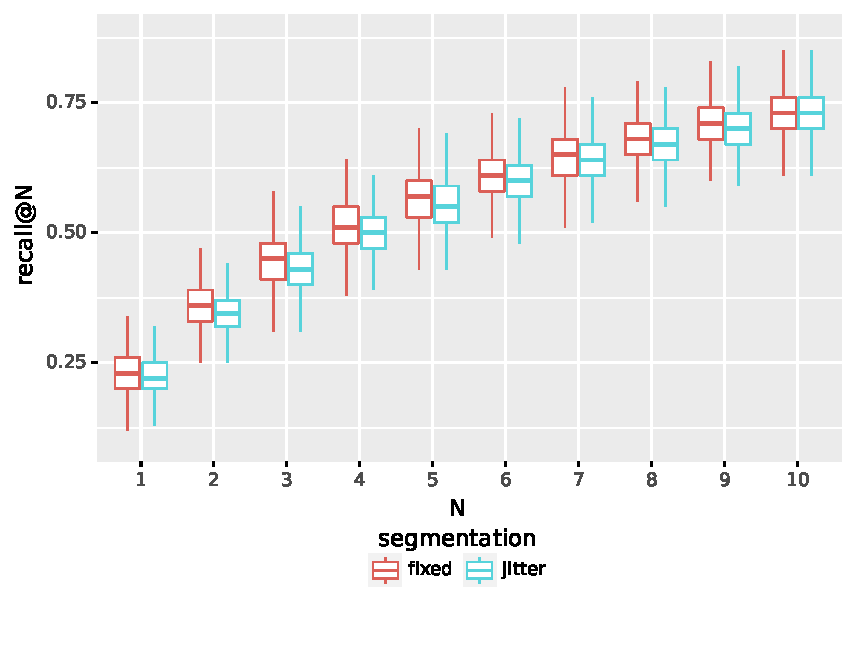
\includegraphics[width=\columnwidth]{results/recall_at_1_to_n_test.pdf}
  \caption{Recall@$N$ as a function of $N$, for the narration test
    data. We show recall for the {\sc fixed} and {\sc jitter}
    retrieval evaluation settings. }
  \label{fig:recall_at_1_to_n}
\end{figure}

\begin{table}[htb]
  \begin{tabular}{lll}
\toprule
R@10 (fixed) & R@10 (jitter) & Triplet Acc \\
\midrule
 0.73 ± 0.05 &   0.73 ± 0.04 & 0.91 ± 0.01 \\
\bottomrule
\end{tabular}

  \caption{Performance of the complete model on narration test
  	data. We show the mean and standard deviation over the
  	bootstrapped scores, pooled over four training runs
	(chance recall@10 = 10\%; chance triplet accuracy = 50\%).}
  \label{tab:test_scores}
\end{table}



\subsection{Ablations}
\label{sec:ablations}
For completeness, we report results on both dialog and narration
data. However, the scores on narration are the main focus as they are
not confounded by speaker-based clues, and thus indicate to what
extent the model learns aspects of utterance meaning.

For experiments in Section~\ref{sec:pretraining} we include each run as a separate boxplot
to show the consistency of the results between runs in
different training conditions.  For the other experiments we collapse
the results of the four runs to avoid clutter.

\subsubsection{Pre-training and Fine-tuning}
\label{sec:pretraining}

Results on different pre-training configurations are shown in
\Cref{fig:pretraining}.
\begin{figure*}[htb]
	\centering
	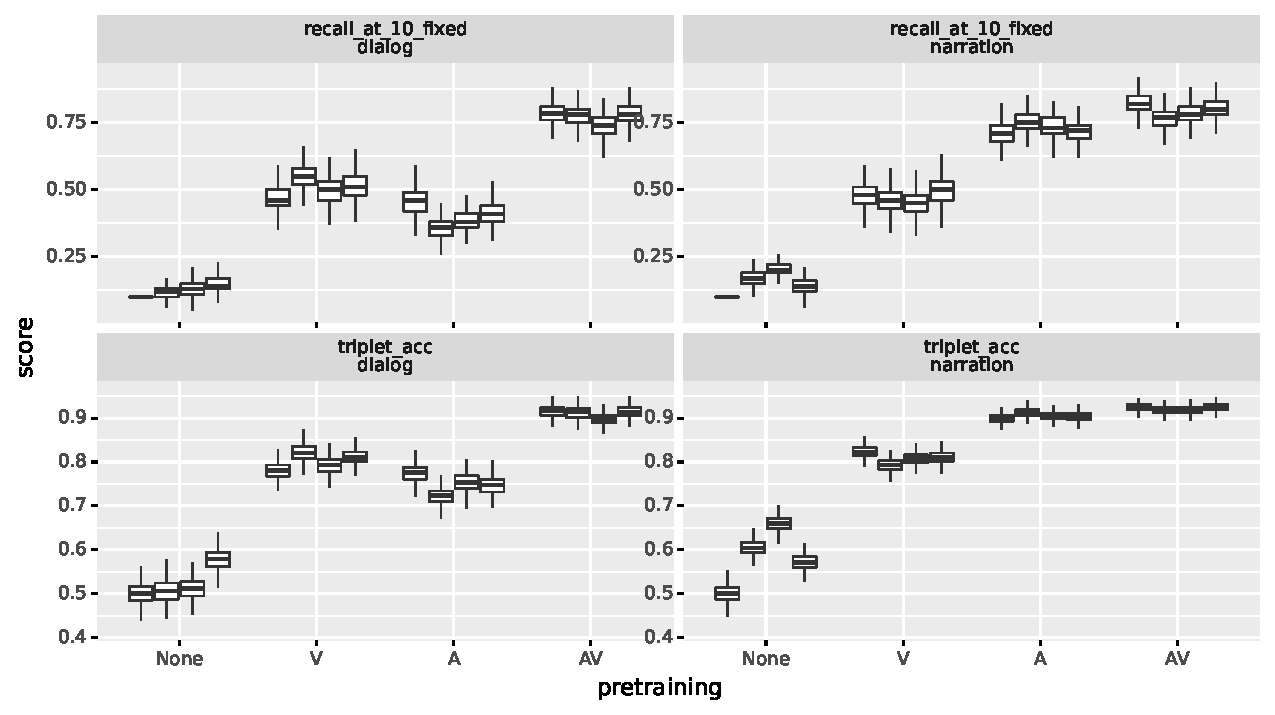
\includegraphics[width=\textwidth]{results/ablations/pretraining.pdf}
	\caption{Effect of pre-training on performance on the dialog
          and narration validation data. The top row shows recall@10
          (chance = 10\%); the bottom row triplet accuracy (chance =
          50\%). Within each condition, we show scores for four
          separate runs. AV: pretrained audio and video; A: pretrained
          audio; V: pretrained video; None: no pretraining.}
	\label{fig:pretraining}
      \end{figure*}

The best overall performance on both the dialog and the narration data is 
achieved with a model where both the video and audio encoder are pre-trained 
before being fine-tuned on our data. On narration data, for both metrics,
we see a clear ranking of
configurations from best to worst: (AV) audio and video pre-training,
(A) audio pre-training, (V) video pre-training and (None) no
trainining. Meanwhile for dialog data, the performance between A and V
is comparable. In the absence of any pre-training (None),
some runs fail to converge, thus performing at chance level.

To further understand and disentangle the effects of audio pre-training and 
fine-tuning, we train a model with frozen parameters of the 
\textsc{wav2vec2} module. The effect of this condition is shown in \Cref{fig:freeze_wav2vec}.
\begin{figure}[htb]
  \centering
  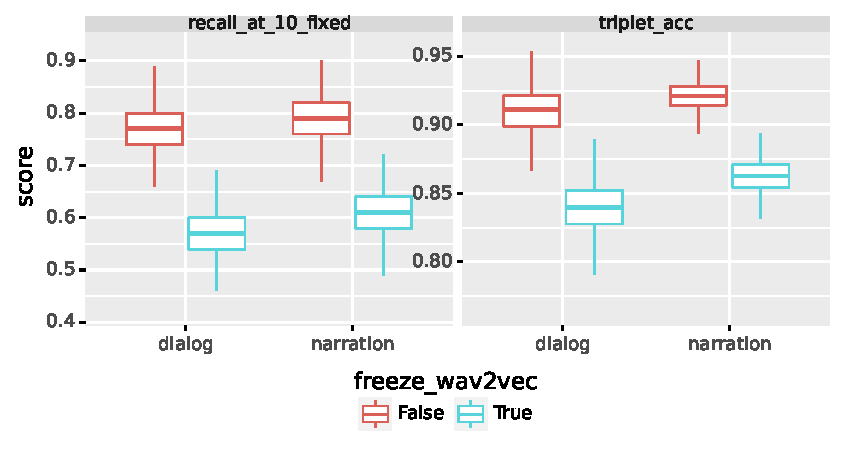
\includegraphics[width=\columnwidth]{results/ablations/freeze_wav2vec.pdf}
  \caption{Effect of freezing the parameters of the \textsc{wav2vec2}
    module on model performance, on the dialog and narration
    validation data (True: \textsc{wav2vec2} frozen; False:
    \textsc{wav2vec2} trained). The top row
    shows recall@10; the bottom row triplet accuracy.}
  \label{fig:freeze_wav2vec}
\end{figure}
We find without fine-tuning of the \textsc{wav2vec2} module, performance 
decreases substantially 
on both metrics. In other words, best performance is only achieved with pre-trained and 
fine-tuned models.


\subsubsection{Jitter}
Next, we evaluate a model that has been trained with varying video and audio 
lengths (\textsc{jitter}). For fair comparison, here we report recall@10 for both 
\textsc{fixed} and \textsc{jitter} validation configurations.
As seen in \Cref{fig:jitter}, the effect of \textsc{jitter} is only
minor and that performance is comparable.
However, we observe 
substantial performance improvements when using \textsc{jitter} in the more 
controlled minimal pairs evaluation (cf. \Cref{sec:minimal-pairs}).
\begin{figure}[htb]
	\centering
	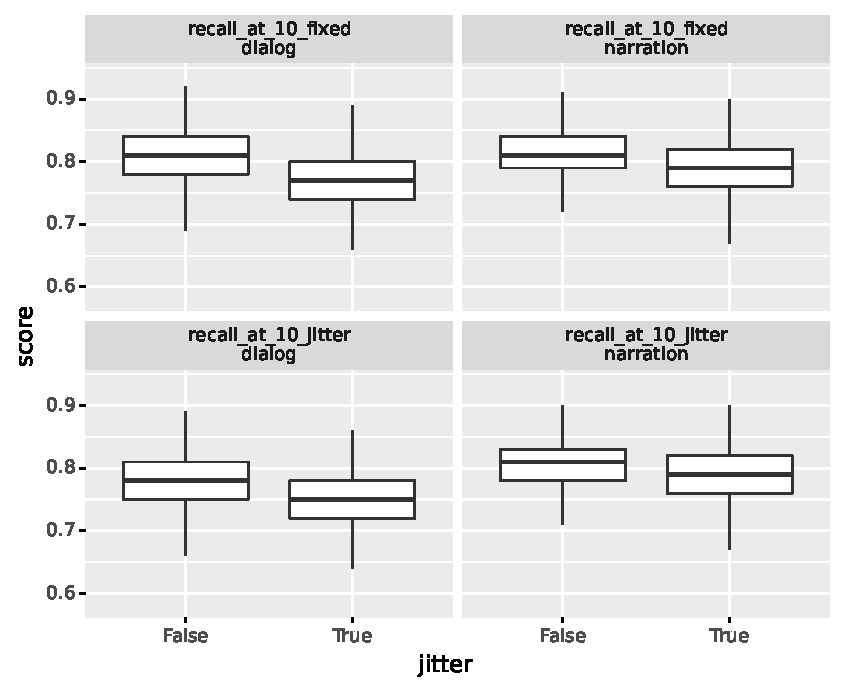
\includegraphics[width=\columnwidth]{results/ablations/jitter.pdf}
	\caption{Effect of jitter on model performance, on the dialog
          and narration validation data (True: jitter; False:
          fixed). The top row shows recall@10 on {\sc fixed}
          evaluation data ; the bottom row on {\sc jitter}-ed data.}
	\label{fig:jitter}
\end{figure}



\subsubsection{Temporal Information}
Finally, we explore the role of the temporal nature of the visual
modality.  \Cref{fig:static} compares the model with the regular video
encoder with one using the \textsc{static} baseline encoder.  For this
comparison we did not pre-train the video encoder in either condition,
in order to remove the confound of the pre-training data.  Across all
metrics, we observe substantial performance drops for the
\textsc{static} model, which has access to the same video frames, but
does not leverage their temporal ordering.
\begin{figure}[htb]
  \centering
  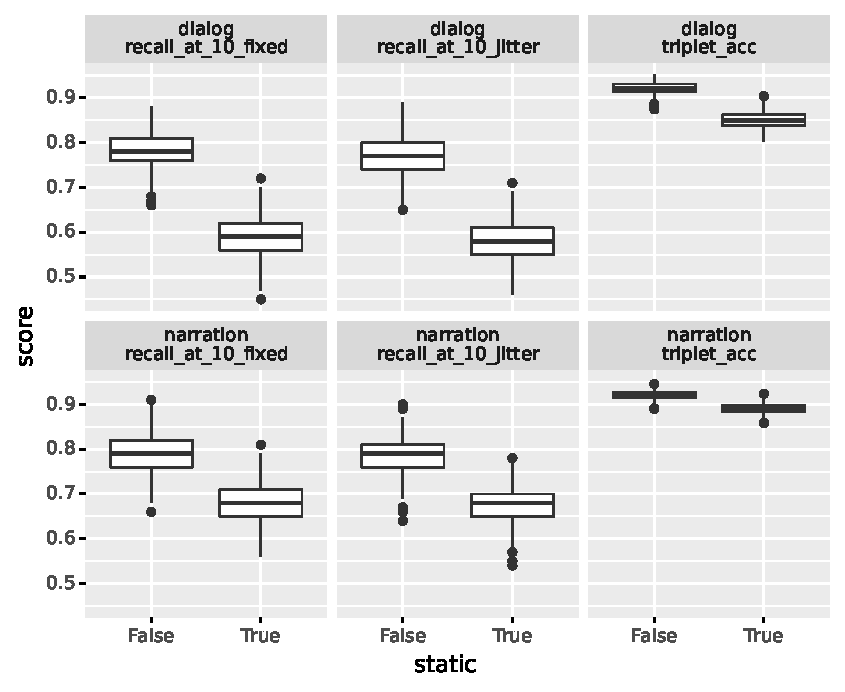
\includegraphics[width=\columnwidth]{results/ablations/static.pdf}
  \caption{Effect of a \textsc{static} image encoder on model
    performance, on the dialog and narration validation data (True:
    static video encoder; False: regular video encoder). The top row
    shows recall@10; the bottom row triplet accuracy.}
  \label{fig:static}
\end{figure}
Additionally we investigate the effect of clip duration on this same
comparison, using the triplet evaluation
data. \Cref{fig:duration_effect} shows that the effect is nonlinear,
and for the shortest clips the access to temporal information does not
help and even has a detrimental effect.

\begin{figure}[htb]
  \centering
  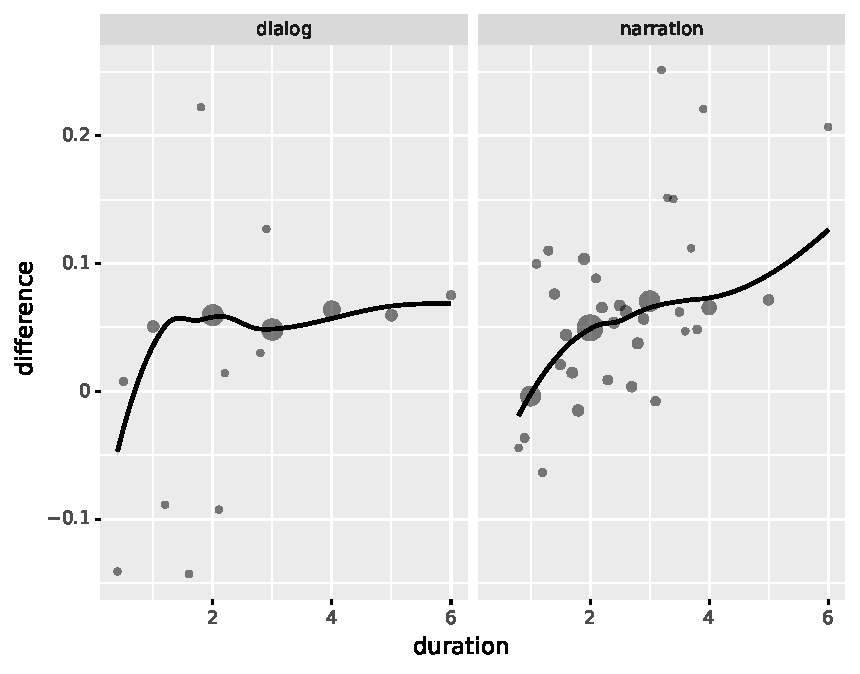
\includegraphics[width=\columnwidth]{results/duration_effect.pdf}
  \caption{The effect of clip duration on the difference in
    performance between models with and without access to temporal
    information, on triplet data. Here we use the undiscretized
    triplet scores (i.e.\ $\mathrm{cosine}(A, P) - \mathrm{cosine}(A,
    N))$, average them over all triplets with the same duration, and
    for each duration compute the difference in the average between
    time-aware and static models. The size of the points corresponds
    to the number of triplets within each duration. The line of fit is
    a loess smoother weighted by size.}
  \label{fig:duration_effect}
\end{figure}

\Cref{fig:scrambled_video} shows the effect of scrambling the video frames 
along the temporal dimension at test time. As expected, we observe substantial 
performance drops when the model does not see the video frames in 
the correct order. 
\begin{figure}[htb]
	\centering
	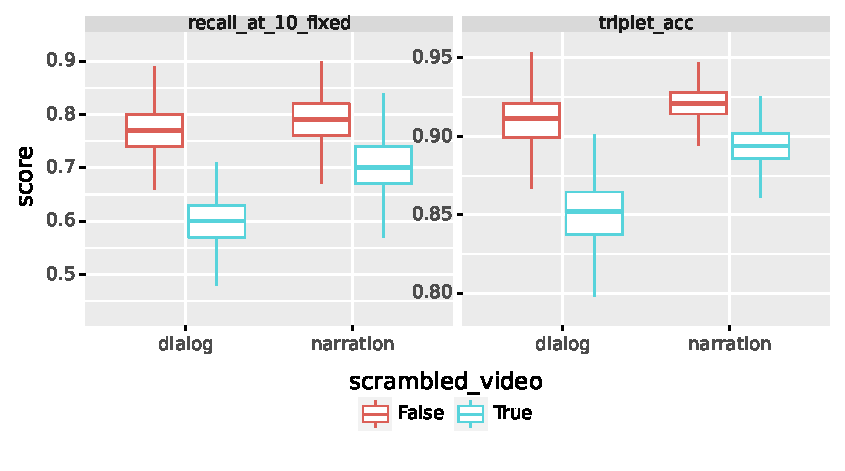
\includegraphics[width=\columnwidth]{results/ablations/scrambled_video.pdf}
	\caption{Effect of scrambling the video frames on model performance, on the 
	dialog and narration validation data (True: video frames scrambled;
        False: video frames in order). The top row shows recall@10;
		the bottom row triplet accuracy.}
	\label{fig:scrambled_video}
\end{figure}
In both experiments the drop in performance due to lack of temporal
information is more acute for the dialog data: this may possibly be due to the
role of the order in which characters speak as a clue in the
dialog segments.

\subsection{Minimal Pairs}
\label{sec:minimal-pairs}


\Cref{tab:minimal_pair_results} presents results for the minimal pair 
evaluation along with several ablations. Models which are 
pre-trained and fine-tuned with \textsc{jitter} (ID 0) perform best. In the 
first two 
configurations (ID~0 and ID~1), there is not much difference in the scores for 
verbs and nouns. 
However, we observe a substantial performance drop for both nouns and verbs if 
the \textsc{wav2vec2} module is not fine-tuned.

If the model is trained without \textsc{jitter} (ID 2), performance drops 
substantially
for nouns, but not for verbs. One possible explanation for this could be that 
the evaluation samples for nouns are on average shorter than those for verbs 
(nouns: $0.43s$ vs. verbs: $0.49s$), and model trained with \textsc{jitter} 
performs better on short clips because it has been exposed to clips of varying 
duration during training. Supporting this hypothesis, we find a positive 
correlation between log duration of clips and accuracy, which is lower for 
models trained with \textsc{jitter} (Pearson $r= 0.52$, $p < 0.001$) than for 
models without \textsc{jitter} (Pearson $r= 0.69$, $p < 0.001$).

In line with the general results, we find that the benefit of audio pretraining 
(ID 5) is greater that that of video pretraining (ID 4). A model without any 
pretraining (ID 3) only performs marginally above chance.

For a model trained with a \textsc{static} video encoder (ID 6), we compare 
performance to a model that was also trained without video pretraining (ID 5) 
as done for the general results. Surprisingly, we observe a slight performance 
improvement for nouns (and no significant difference for verbs).\footnote{One 
reason for this counterintuitive performance improvement could be other aspects 
of the architectures of the compared video encoders. For example, the 
\textsc{static} video encoder leverages only 11,7M parameters, while the 
normal video encoder has 31,5M parameters. The increased number of parameters 
could cause the model to overfit more to the training data.} We hypothesize 
that temporal information is not crucial for the minimal pairs evaluation, 
because most evaluation samples are clips of short duration (on average: 
$0.44s$, i.e. 4-5 frames), thus limiting the benefit of temporal information.
As we could observe in the analysis of clip duration 
(\Cref{fig:duration_effect}), temporal information for such short clips does 
not improve performance, and could even have detrimental effects.
In the alternative temporal ablation with scrambled video frames (ID 7), we 
observe no significant performance drop compared to the top condition (ID 
0).
\begin{table*}[htb]
	\centering
	\begin{tabular}{lllll}
\toprule
     Finet &       Jitt &        Tmp &      Nouns &      Verbs \\
\midrule
\checkmark & \checkmark & \checkmark & 0.81±0.002 & 0.81±0.007 \\
           & \checkmark & \checkmark & 0.71±0.002 & 0.69±0.006 \\
\checkmark &            & \checkmark & 0.73±0.003 & 0.79±0.006 \\
\checkmark & \checkmark &            & 0.79±0.002 & 0.77±0.007 \\
\bottomrule
\end{tabular}

	\caption{Minimal pair accuracies for nouns and verbs for different model 
		ablations. W2V Finet: \textsc{wav2vec2} module finetuned; A Pretr: 
		Audio encoder pretrained; V Pretr: Video encoder pretrained; Tmp 
		Enc: Video encoder with temporal information (not \textsc{static}); 
		Tmp Frames: Video frames in correct temporal order (not scrambled). 
		Mean and standard 
		deviation calculated over bootstrapped scores (100 re-samples), pooled 
		over 4 training runs.}
	\label{tab:minimal_pair_results}
\end{table*}


\begin{figure}[htb]
  \centering
  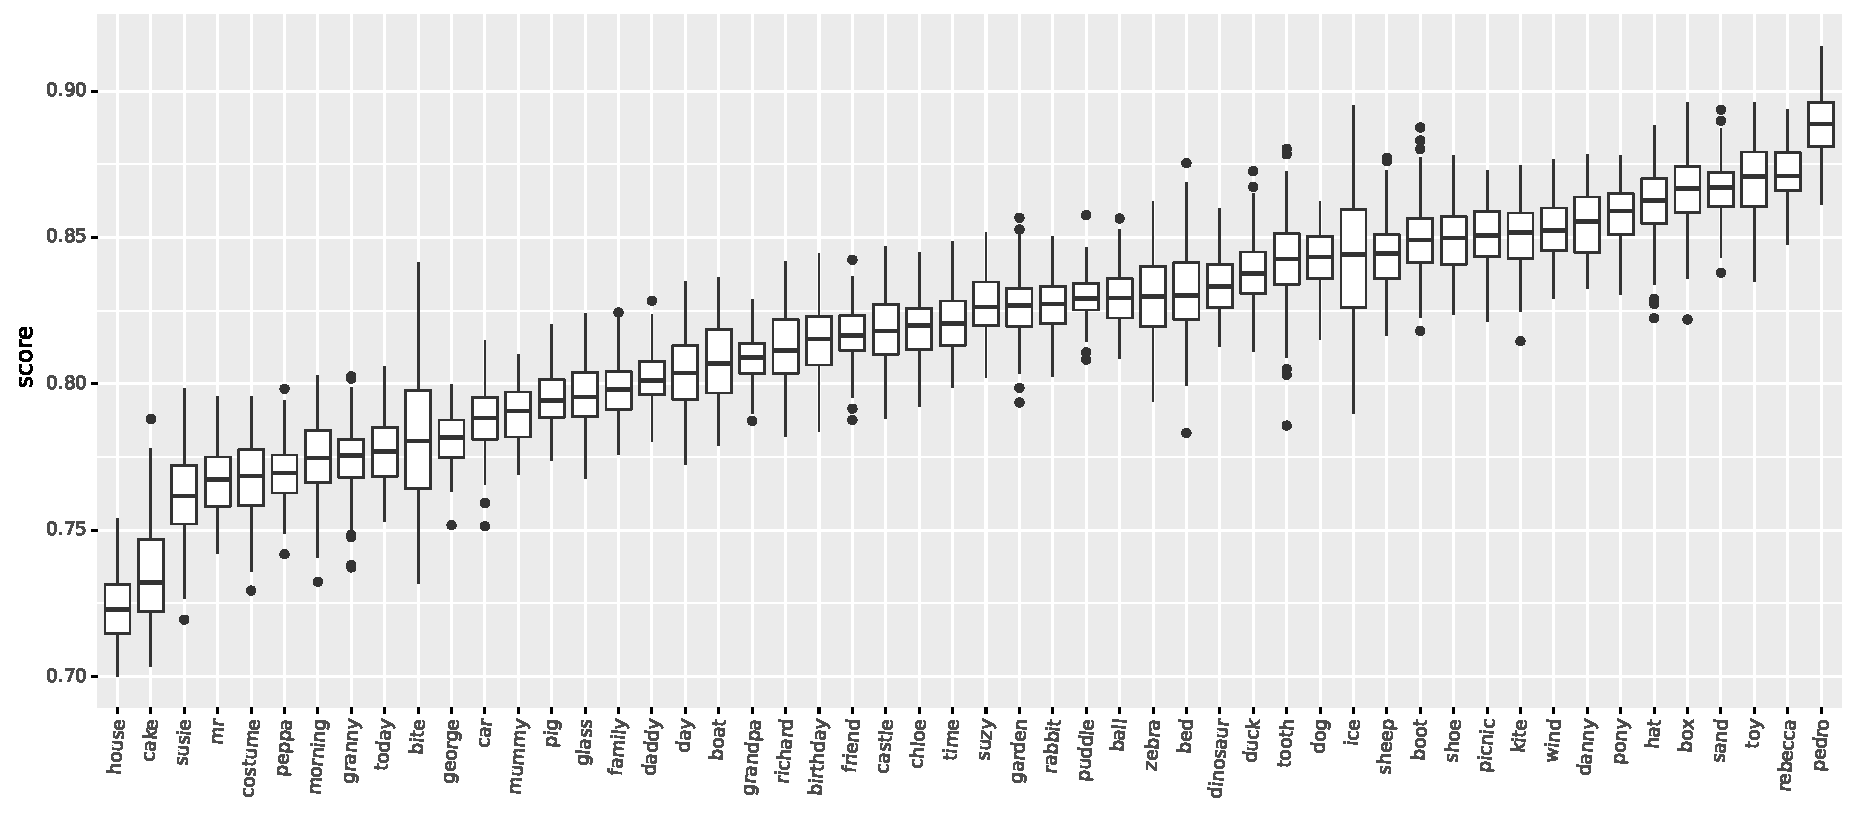
\includegraphics[width=.5\textwidth]{results/targeted_triplets/acc_per_word_NOUN.pdf}
  \caption{Per-word accuracies on the minimal pairs evaluation data for nouns.}
  \label{fig:accuracy_targeted_triplets_nouns}
\end{figure}

\Cref{fig:accuracy_targeted_triplets_nouns} shows per-word
accuracy for nouns for the best performing model configuration.
We observe substantial variance in the accuracy scores, suggesting that the 
difficulty to learn certain words varies. For example, the 
scores for \textit{house}, \textit{car}, and \textit{cake} are the lowest. This could be 
because these concepts are not easy to ground, either because they are used in 
displaced speech or because they do not often refer to a similar visual entity. 
When looking at our evaluation samples, we find that indeed the word \textit{house} 
is used in varying visual contexts (house entrance, whole house, inside the
house, rabbit's house) and in displaced speech (talking about going 
to somebody's house). Cars are only sometimes completely visible, often we see 
only pigs \textit{in} a car. Regarding \textit{cake}, it refers to either a 
whole cake, a slice, dough, or crumbs.

On the other end, performance for concrete words such as \textit{ice}, 
\textit{box}, 
and \textit{sand} is the best, and indeed we find that in the evaluation examples 
these concepts are always present in the corresponding video and visually 
highly similar. Additionally, the words \textit{Pedro}, and \textit{Rebecca} 
are learned very well: They refer to \textit{Pedro Pony} and \textit{Rebecca Rabbit}, 
easily visually distinguishable from characters belonging to other species.

Further investigations with larger datasets are necessary to reveal the 
underlying reasons for difficulty, and relating them to predictors of age of 
acquisition in the child language acquisition literature 
\cite{roy2015predicting,frank2021variability}. 


